%Alle zu bearbeitenden Felder sind als solche gekennzeichnet. 
%Warnungen sind in der Regel nicht komplett vermeidbar und auch in dieser Vorlage vorhanden (Bei mir 7). Sie sind meistens eher als Hinweise zu verstehen.
%Bei Fragen zu dieser Vorlage einfach eine Mail an gold@lfe.mw.tum.de
%Viel Erfolg!


\documentclass[
	12pt,
	headinclude,
	footinclude,
	a4paper,
	listof=totoc,
	bibliography=totoc,
	index=totoc,
	%twoside, %F�r beidseitigen Druck
	]{scrreprt}


	
	
\newcommand{\myname}[0]{Max Mustermann} %---------- HIER NAME EINTRAGEN ----------
\newcommand{\mythema}[0]{Titel der Studienarbeit} %---------- HIER TITEL EINTRAGEN ----------
\newcommand{\mythemaeng}[0]{Titel der Studienarbeit in Englisch} %---------- HIER TITEL IN ENGLISCH EINTRAGEN ----------
\newcommand{\myarbeit}[0]{Interdisciplinary Project} %---------- HIER ART DER ARBEIT EINTRAGEN ----------
\newcommand{\mymodul}[0]{Produktionstechnik} %---------- HIER STUDIENGANGMODUL EINTRAGEN ----------

%----- Bitte au�erdem die Datei _names.tex anpassen ------


\usepackage[
%headinclude, 
%footinclude,
%headsepline,
%footsepline,
%plainfootsepline, 
%plainheadsepline,
automark
]{scrpage2}



\pagestyle{scrheadings}
\clearscrplain
\clearscrheadings
\ofoot[\pagemark]{\pagemark} %Seitenzahlen rechts unten, bitte!
\addtolength{\footskip}{-1cm} %Seitenzahlen ein bisschen h�her setzen


\newcommand{\bild}[4]{
  \begin{figure}[!hbt]
    \begin{center}
    %\centering
      %\vspace{1ex}
      \includegraphics[#2]{img/#1}
      \caption[#4]{\label{img.#1} #3}
    \end{center}
    %\vspace{1ex}
  \end{figure}
 }
 
%bild mit rahmen 
\newcommand{\rbild}[4]{
  \begin{figure}[!hbt]
    \begin{center}
    \fbox{
    %\centering
      %\vspace{1ex}
      \includegraphics[#2]{img/#1}
      }
      \caption[#4]{\label{img.#1} #3}
    \end{center}
    %\vspace{1ex}
  \end{figure}
 }
 
 

\newcommand{\fbild}[5]{
  \begin{floatingfigure}[r]{#5}
    \begin{center}
    %\centering
      %\vspace{1ex}
      \includegraphics[#2]{img/#1}
      \caption[#4]{\label{img.#1} #3}
    \end{center}
    %\vspace{1ex}
  \end{floatingfigure}
 }


\newcommand{\mytab}[4]{
    \begin{table}[!hbt]
    \begin{center}
      \vspace{1ex}
		\begin{tabular}{#2}
			\hline %hline here beacuse hline as first command in included \input-files produces errors
			    \input{tab/#1}
			\hline	    		
		\end{tabular}
          \caption[#4]{\label{tab.#1} #3}
    \end{center}
    \vspace{1ex}
\end{table}
}

\newcommand{\tausend}{\hspace {.5ex}} %50\t 000 => 50 000 tausender trenner 

\newcommand{\comment}[1]{} 

\newcommand{\mytabsmall}[4]{
    \begin{table}[!hbt]
    \begin{center}
      \vspace{1ex}
      {\tiny
		\begin{tabular}{#2}
			\hline %hline here beacuse hline as first command in included \input-files produces errors
			    \input{tab/#1}		
			\hline
		\end{tabular}
		}
          \caption[#4]{\label{tab.#1} #3}
    \end{center}
    \vspace{1ex}
\end{table}
}


% foldersymbol
\newcommand{\folder}[1]{
      \hspace{-3ex}
 \scalebox{0.40}[0.40]
{\includegraphics[viewport=14 15 48 48,clip]{img/folder.pdf}  }
 \bf #1 \normalfont \tiny
 }

% dokumentsymbol 
\newcommand{\dokument}[1]{
      \hspace{-3ex}
 \scalebox{0.60}[0.50]
{\includegraphics[viewport= 22 16 40 42, clip]{img/dokument.pdf}  }
 \bf #1 \normalfont \tiny
 }

% ANWENDUNGSBEISPIELE--------------------------------------------------------------------
%    \bild{meinbild.pdf}{viewport=0 0 200 350, clip=true}{BILDUNTERSCHRIFT}{Eintrag fuers Abbildungsverzeichniss}
%    \bildscale{meinbild.pdf}{viewport=0 0 200 350, clip=true}{BILDUNTERSCHRIFT}{Eintrag fuers 
% 																																									Abbildungsverzeichniss}{scalex}{scaley}
%    \mytab{datei_in_der_die_tabelle_ist.tex}{lrrr <= Format }{TABELLENUNTERSCHRIFT}{Eintrag fuers Tabellenverzeichnis}
%    \dokument[datei$.$mat] % punkt maskieren '$.$' wegen 'dirtree'-umgebung
%    \folder[mydirectory]



% macht den rand schoener (optischer randausgleich)
\usepackage[activate=normal]{pdfcprot}


\usepackage{units}
%\unit[Wert]{Einheit}
%\unitfrac[Wert]{Z�hler}{Nenner}

\newcommand{\myunit}[1]{\,\unit{#1}}  % ohne []
\newcommand{\myunitrm}[1]{\,\mathrm{\unit{#1}}} % mit []
\newcommand{\myunitfrac}[2]{\,\mathrm{\unitfrac{#1}{#2}}}
%
%U = 2.459\, 123 \myunit{V}
%\sigma = \frac{F}{A} = 133.432\, 192\, 233 \myunitfrac{N}{mm^{2}}

\usepackage{url}

\usepackage[plainpages=false,pdfpagelabels=true,bookmarks=true, 
						%bookmarksopen=true, % waehrend testen offen lassen spaeter zumachen
						pdfpagemode={UseOutlines},pdfstartview={FitV},pdfborder={0 0 0},
						pdfauthor={\myname}, 
						pdftitle={\mythema},
						%pdfsubject={\mythema}, % optional
						%pdfkeywords={Schluesselwort1,Schluesselwort2,Schluesselwort3},
						colorlinks=true,
						linkcolor=black,
						filecolor=black,
						urlcolor=black,
						citecolor=black,
						hypertexnames=true,
						pdfpagelabels=true,
						hyperindex=true,
						linktocpage=true,
						pagebackref=true
						]{hyperref}
						
						

	\usepackage[round]{natbib}
    \usepackage{amsmath} 
    \usepackage{dirtree}
    \usepackage{algorithm}
    \usepackage[noend]{algpseudocode}
    \usepackage{subcaption}
	\usepackage{geometry}
%	\geometry{left=3.5cm,textwidth=15cm,top=2.5cm,textheight=24.5cm}
%	\geometry{left=2.5cm, right=2.5cm, bottom=3cm, top=2.5cm}
	\geometry{left=3cm, right=2.6cm, bottom=3cm, top=2.5cm}
	
	\usepackage{makeidx}
	\makeindex

\usepackage{setspace}
%\onehalfspacing %Zu klein im Vergleich zu Word
\setstretch{1.54} %Simuliert den 1,5 fachen Zeilenabstand von Word (Bei dieser Schriftart und dieser Schriftgr��e)
\renewcommand{\arraystretch}{1.54} %Zeilenabstand in Tabellen! 

\setlength{\parindent}{0pt} %Kein Einr�cken der ersten Zeile eines Absatzes
\setlength{\headheight}{1.1\baselineskip}

\usepackage{titlesec} %Dieser Abschnitt definiert die �berschriften
\titleformat{\chapter}[block]{\large\bfseries}{\thechapter}{.5em}{}
\titleformat{\section}[block]{\large\bfseries}{\thesection}{.5em}{}
\titleformat{\subsection}[block]{\large\bfseries}{\thesubsection}{.5em}{}
\titleformat{\subsubsection}[block]{\large\bfseries}{\thesubsubsection}{.5em}{}

%
%
%\setlength{\headsep}{1cm}
%\setkomafont{pagefoot}{\normalfont} %Sonst wird Fu�zeile kursiv
%\setkomafont{pageheadfoot}{\normalfont} %Sonst wird Kopfzeile kursiv
%
%%\pagestyle{scrheadings}
\clearscrheadfoot % clear header and footer
%\automark[section]{chapter}
%\ihead[]{\leftmark} % header left part
%%\ohead[]{\rightmark} % header right part
%\ohead[]{\scalebox{0.05}{\includegraphics{img/lfe.pdf}}} % header right part
%\ifoot{\small \myarbeit \space \myname} % footer left part  
%%\cfoot{\vspace{-0.5cm}\mythema} % footer middle part
%%\ofoot{Seite\ {\pnumfont \pagemark}\ von {\pnumfont \pageref{LastPage}}} % footer right part
\ofoot{\small {\pnumfont \pagemark}} % footer right part
%\setheadsepline{0.3pt} % set header seperate line
%\setfootsepline{0.3pt} % set footer seperate line
%%\setheadwidth{textwithmarginpar}
%%\setfootwidth{textwithmarginpar}



\usepackage[dvips]{graphicx}
\usepackage{floatflt,epsfig} 

% \usepackage{ngerman} % neue deutsche Rechtschreibung
% \usepackage[latin1]{inputenc} % latin1-Kodierung f�r Umlaute
% \usepackage[ngerman]{babel}  % Silbentrennung
\usepackage[T1]{fontenc}
\usepackage[scaled]{uarial} % Schriftart Arial
\usepackage[font=small,labelfont=it]{caption} %�berschriften kursiv


\renewcommand*\familydefault{\sfdefault} %Sonst werden die Header nicht in der entsprechenden Schriftart dargestellt
\renewcommand\thefigure{\arabic{chapter}-\arabic{figure}} %Nummerierung der Abbildungen mit - statt .
\renewcommand\thetable{\arabic{chapter}-\arabic{table}} %Nummerierung der Tabellen mit - statt .

\setcounter{secnumdepth}{3} %Tiefe der Numerierung
\setcounter{tocdepth}{3} %Tiefe des Inhaltsverzeichnisses
\usepackage{graphicx}

\clubpenalty = 10000 % Schusterjungen vermeiden
\widowpenalty = 10000 % Hurenkinder vermeiden
\displaywidowpenalty = 10000 % und nochmal f�r Formeln

\usepackage{graphicx} % Bilder
\usepackage{color} % Farben
\usepackage{colortbl} % tabellen einf�rben
\usepackage{floatflt} % graphiken mit textumfluss
% \usepackage{subfigure} % graphiken nebeneinander mit (a) (b)
\usepackage[absolute]{textpos} % absolute positioning


\usepackage{scrhack}
\usepackage{listings} % programmcode als listings darstellen

%workaround
% \addto\captionsngerman{
%  \renewcommand{\figurename}{Abbildung}%
% }

 %Definition zu Bildern und Dokumentstyle



% --------------------------------------------------
% -------------------- DOCUMENT --------------------
% --------------------------------------------------


\begin{document}


\thispagestyle{empty} %Keine Seitennummer auf der Titelseite

\begin{picture}(0,0) 
   \put(-8,0){
   
			\begin{minipage}[ht]{0.3\textwidth}
			\centering
			\includegraphics[width=2.5cm]{img/lfe.pdf}
			\end{minipage}
   
%   } 

   \hspace{7cm}
   
   %\put(0,0){
			\begin{minipage}[ht]{0.3\textwidth}
			\centering
			\includegraphics[width=2.3cm]{img/tum.png}
			\end{minipage}
	}   
\end{picture} \\


\ \\
Technische Universit�t M�nchen\\
Lehrstuhl f�r Ergonomie 


\vspace{5cm}

{\large\bf \myarbeit}\\

\vspace{1cm}

{\Large\bf \mythema}\\

{\large\bf \mythemaeng}


\vspace{3cm}


{\large\bf \myname}\\


 %Titelseite, wird automatisch erstellt

\renewcommand{\thepage}{\roman{page}} %R�mische Zahlen von Hauptteil

\clearpage

\begin{picture}(0,0) 
   \put(-8,0){
   
			\begin{minipage}[ht]{0.3\textwidth}
			\centering
			\includegraphics[width=2.5cm]{img/lfe.pdf}
			\end{minipage}
   
%   } 

   \hspace{7cm}
   
   %\put(0,0){
			\begin{minipage}[ht]{0.3\textwidth}
			\centering
			\includegraphics[width=2.3cm]{img/tum.png}
			\end{minipage}
	}   
\end{picture} \\


\ \\
Technische Universit�t M�nchen\\
Lehrstuhl f�r Ergonomie 

\vspace{3cm}


{\Large\bf \mythema}\\

{\large\bf \mythemaeng}\\

\vspace{1cm}

{\large \myarbeit}\\

\vspace{1cm}


\begin{table}[!hbt]
\large
		\begin{tabular}{ll}
      \vspace{0.5cm}
				Verfasser: & \myname\\
      \vspace{0.5cm}
				Module: & \mymodul\\
      \vspace{0cm}
				Betreuer:	&Univ.-Prof. Dr. phil. Klaus Bengler\\
			\vspace{0cm}
									&Dipl.-Ing. N. N.\\
			\vspace{0.5cm}
									&Dipl.-Inf. N. N.\\						
      \vspace{0.5cm}
				Ausgabe am:&01.01.2012\\
      \vspace{0.5cm}
				Abgabe am:&30.06.2012\\    		
		\end{tabular}
    \vspace{1ex}
\end{table}

 %---------- Bitte anpassen! ----------

\clearpage

\noindent{\Large\bf Eidesstattliche Erkl�rung }\\
\\
Hiermit versichere ich diese Studienarbeit ohne fremde Hilfe selbst�ndig verfasst und nur die angegebenen Quellen und Hilfsmittel verwendet zu haben. W�rtlich oder dem Sinn nach aus anderen Werken entnommene Stellen sind unter Angabe der Quellen kenntlich gemacht.\\
\\
Garching, den\vspace{2.5cm}\\\myname\\

\vspace{3cm}

\noindent{\Large\bf Vereinbarung zum Urheberrecht}\\
\\
Hiermit gestatte ich dem Lehrstuhl f�r Ergonomie diese Studienarbeit bzw. Teile davon nach eigenem Ermessen an Dritte weiterzugeben, zu ver�ffentlichen oder anderweitig zu nutzen. Mein pers�nliches Urheberrecht ist �ber diese Regelung hinaus nicht beeintr�chtigt. 

Eventuelle Geheimhaltungsvereinbarungen �ber den Inhalt der Arbeit zwischen mir bzw. dem Lehrstuhl f�r Ergonomie und Dritten bleiben von dieser Vereinbarung unber�hrt.\\
\\
Garching, den\vspace{2cm}\\\myname
 %Erkl�rungen, wird automatisch erstellt




% --------------------------------------------------
% -------------------- ABSTRACT --------------------
% --------------------------------------------------



\begin{abstract}
\thispagestyle{plain} %F�gt eine Seitenzahl ein
\ofoot[\pagemark]{\pagemark} %F�gt eine Seitenzahl ein

\noindent{\bf Kurzfassung / Abstract}\\


Ein Abstract ist eine pr�gnante Inhaltsangabe, ein Abriss ohne Interpretation und Wertung einer wissenschaftlichen Arbeit. In DIN 1426 wird das (oder auch der) Abstract als Kurzreferat zur Inhaltsangabe beschrieben.

Die Definition des American National Standards Institute (ANSI) lautet: "An abstract is defined as an abbreviated accurate representation of the contents of a document." ("Ein Abstract ist definiert als eine gek�rzte pr�zise Darstellung des Inhalts eines Dokuments.")


\end{abstract}




% --------------------------------------------------
% --------------- INHALTVERZEICHNIS ----------------
% --------------------------------------------------



\tableofcontents %Bindet das Inhaltsverzeichnis ein

\thispagestyle{plain} %F�gt eine Seitenzahl ein
\ofoot[\pagemark]{\pagemark} %F�gt eine Seitenzahl ein

\clearpage

\phantomsection

\clearpage

\setcounter{page}{4} %Seitenz�hler resetten

% --------------------------------------------------
% ------------------- HAUPTTEIL --------------------
% --------------------------------------------------



\newpage{\pagestyle{plain}
\cleardoublepage}
\renewcommand{\thepage}{\arabic{page}}
\setcounter{page}{1}
\pagestyle{scrheadings}
\renewcommand*{\chapterpagestyle}{scrheadings}

%Es bietet sich an, die einzelnen Kapitel in eigene *.tex Dateien auszulagern, um die �bersichtlichkeit zu verbessern. Sollte das nicht gew�nscht sein, k�nnen die Inhalte dieser *.tex Dateien hier eingef�gt und die "\input xxx.tex"' zeilen entfernt werden.
%Die Gliederung/Kapitel ist/sind nat�rlich der Arbeit entsprechend anzupassen

\chapter{Introduction} \label{cha:introduction}

In the development of new interfaces for the vehicles, or simply in the study of 
the influence in driving performance of some factor of interest, an evaluation
has to be performed. There are different ways to measure the driving quality of
a person under the interest conditions. In particular, there are two important
measurements for this task, the Time to Headway (THW) and the standard deviation
of lateral position (SDLP).

To calculate these measurements is necessary to use points of reference. In the
case of the Time to Headway the point of reference are the vehicles driving in
front of the testing car. In the case of the SDLP measurement, the lanes on the
road are used as the reference point to obtain the lateral position.

In a virtual environment is easy to obtain the exact position of the vehicles
and the lanes on the road, but in the real world is not an easy task. In real
world applications, sensors are used to estimate the position of these reference
points. Unfortunately, sensor measurements generally have some error associated
which is directly associated to the price of the sensor. Expensive sensors like
for example laser scanners are very accurate for distance calculation but at the
same time their price is very high. On the other hand, normal color cameras are
getting more popular to be used as sensors in real world reconstruction due to
its low cost and the recent advances in Computer Vision and Image Processing.

In particular, in the recent years a great number of applications using the
Smartphones cameras have been created. For example, augmented reality
applications that superpose a virtual environment by building references with
the real world through the camera.

Here is where the idea of using a similar application for the problem of
evaluating the driving quality shows up. In particular, to create an application
that uses the camera together with Computer Vision technique to calculate the
THW and SDLP measurements in real-time.

This project is precisely this idea taken to practice. We develop an application
for the Android operative system used by Smartphines and mobile devices that
calculate these two measurements. The project was divided in two modules, one
for each measurement. The first one is the Vehicle Detection Module and is the
one responsible for calculate the THW. The second one is called Lane Detection
Module and is the responsible for the detection of the road lanes and the SDLP
calculation.



\chapter{Anmerkungen zum Format} \label{kap:anmerkungen}


Tabelle \ref{tbl:tab1} zeigt, dass Tabellen eine kursive �berschrift tagen.


\begin{table}[h]
	\centering
	\caption{\textit{So sieht eine Tabelle aus (Bild)}}
\includegraphics[width=11cm]{img/tabelle.png}
\label{tbl:tab1}
\end{table} 

Tabellen k�nnen entweder als Bild (z.b. aus Excel) eingef�gt werden oder manuell mit LaTeX erstellt werden (siehe \ref{tbl:tab2}):


\begin{table}[h]
	\centering
	\caption{\textit{So sieht eine Tabelle aus (LaTeX)}}	
	\begin{tabular}{|p{3cm}|p{5cm}|}
 			\hline
			\textbf{Parameter} & \textbf{Kenngr��e}\\
			\hline	
				Schriftgr��e & Arial, Standard, 12 pt\\
				Ausrichtung & Blocksatz mit automatischer Silbentrennung\\
				Zeilenabstand & 1,5\\
			\hline
			\end{tabular}
	\label{tbl:tab2}
\end{table} 


Abbildungen tragen eine kursive Bildunterschrift, wie in Abb. \ref{fig:bild1} zu erkennen.

\begin{figure}[ht]
	\centering
\includegraphics[width=8cm]{img/abbildung.png}
\caption{\textit{So sieht eine Abbildung aus}}
\label{fig:bild1}
\end{figure} 

Verweise auf Kapitel, Tabellen oder Abbildungen mit $\backslash ref\{label\}$.



\chapter{Sumatra PDF Viewer}  \label{kap:sumatra}

Statt den Adobe Reader zu verwenden, bietet sich f�r die Arbeit mit TeXnicCenter der Sumatra PDF-Viewer an. Dieser erm�glicht es, das PDF-Dokument w�hrend der Bearbeitung mit TeXnicCenter ge�ffnet zu lassen. Das PDF-Dokument aktuallisiert sich au�erdem nach der Ausgabe automatisch und die Ansicht bleibt an der entsprechenden Stelle im Dokument.\\

Der Sumatra PDF Viewer ist Freeware und sehr schlank.
Er liegt dieser Vorlage als "SumatraPDF-2.1.1-install.exe" bei, oder steht
auf der Seite des Herstellers zum Download bereit:\\

http://blog.kowalczyk.info/software/sumatrapdf/download-free-pdf-viewer-de.html \\

Nach der Installation muss noch die Einstellung des TeXnixCenter f�r die Verwendung von Sumatra angepasst werden.

Eine Anleitung findet sich in "Sumatra Einrichtung.pdf" oder hier:\\

http://www.texniccenter.org/resources/tutorials


\chapter{Vehicle Detection Module}  \label{kap:vehicle-detection}

\section{Classification refinement} % (fold)
\label{sec:Classification-refinement}

Due to the great spectrum of different textures appearing in an image, false
classification may occur. This is essentially an inherent problem of the
effort the classifier does to predict unknown data. These mistakes from the
classifier are divided into two types, false positives and false negatives. A
false positives occur when the classifier wrongly label negative examples as 
positive and false negatives is the other way around.

Sometimes it is possible to use some strategies to improve a classification by
removing some of this false classifications. In this particular project, we have
the advantage to work with a continuous flow of images coming from a camera.
This fact offers an extra dimension which allow us to make assumptions in
order to filter some of the false classifications.

Basically we assume the camera is fixed inside the vehicle, meaning that the images
coming from it should show always the frontal view. This summed to the stream of
images allow us to suppose that a vehicle appearing in one image is going to also 
appear in the next one, in almost the same region inside the image.

With this in mind, it is easy to design a simple strategy to eliminate some
false positives. Supposing a vehicle can not simply disappear from one
frame to the other, we can construct a classification window over time, where we
keep track of the position of all the previous classified vehicles. If a new
classification is not consistent with the previous ones in the window, then it
is simply dropped. 

The final size of the region containing the vehicle is averaged with the
information inside the classification window. This smooths jumps of the region
size returned by the classifier due to the search in different scales.

% section Classification refinement (end)


\section{Distance estimation} % (fold)
\label{sec:Distance-estimation}

When projecting the real 3D world through the lenses of a camera into a 2D
image, some information is lost. In particular, the scale and the notion of
distances is lost. It is not possible give any real
measurement of distances in the real world just looking at one image. 
Of course, as humans we can find references in an image of something we already
know and stablish some scale to compare the rest of the image. Think for
example of a picture of a small toy car. If the model of this toy car is good 
enough, a human can not differentiate it from a real one, then having an
incorrect estimate of its size.

This is the problem faced in this section and of course, it is required to do some
assumptions to be able to approximate a solution. First it is assumed, that the
pictures obtained from the camera are from real vehicles, this is really
important to build references with of real world distances. Now, this brings a
second problem, that not all the vehicles have the same size. 
The easy solution is to make a second assumption and consider an average width
of all the vehicles appearing in the images.

The third problem is that the width in meters of the vehicles is not obtained 
directly from the picture, but a group of pixels containing the image of
the car. To solve this, is necessary to find the relation between the number of
pixels containing the car, and the distance to it. For this reason, as a first
approach, a number of pictures at different distances of a car where taken. This
pictures appear in the figure [inser figure here].

In the figure~\ref{fig:distance-curve-fitting} are displayed as red points, the
measurements obtained from each image. As you can see, this points follows an
exponential function. In order to be able to make a prediction of the distance,
it was decided to fit a exponential model to this data points. The exponential
model selected for this task is given by the next formula

\begin{equation}
    \mathcal{M}(x) = a \cdot \exp(b \cdot x) + c \cdot \exp(d \cdot x)
    \label{eq:distance-curve-model}
\end{equation}

\begin{figure}[h]
\centering
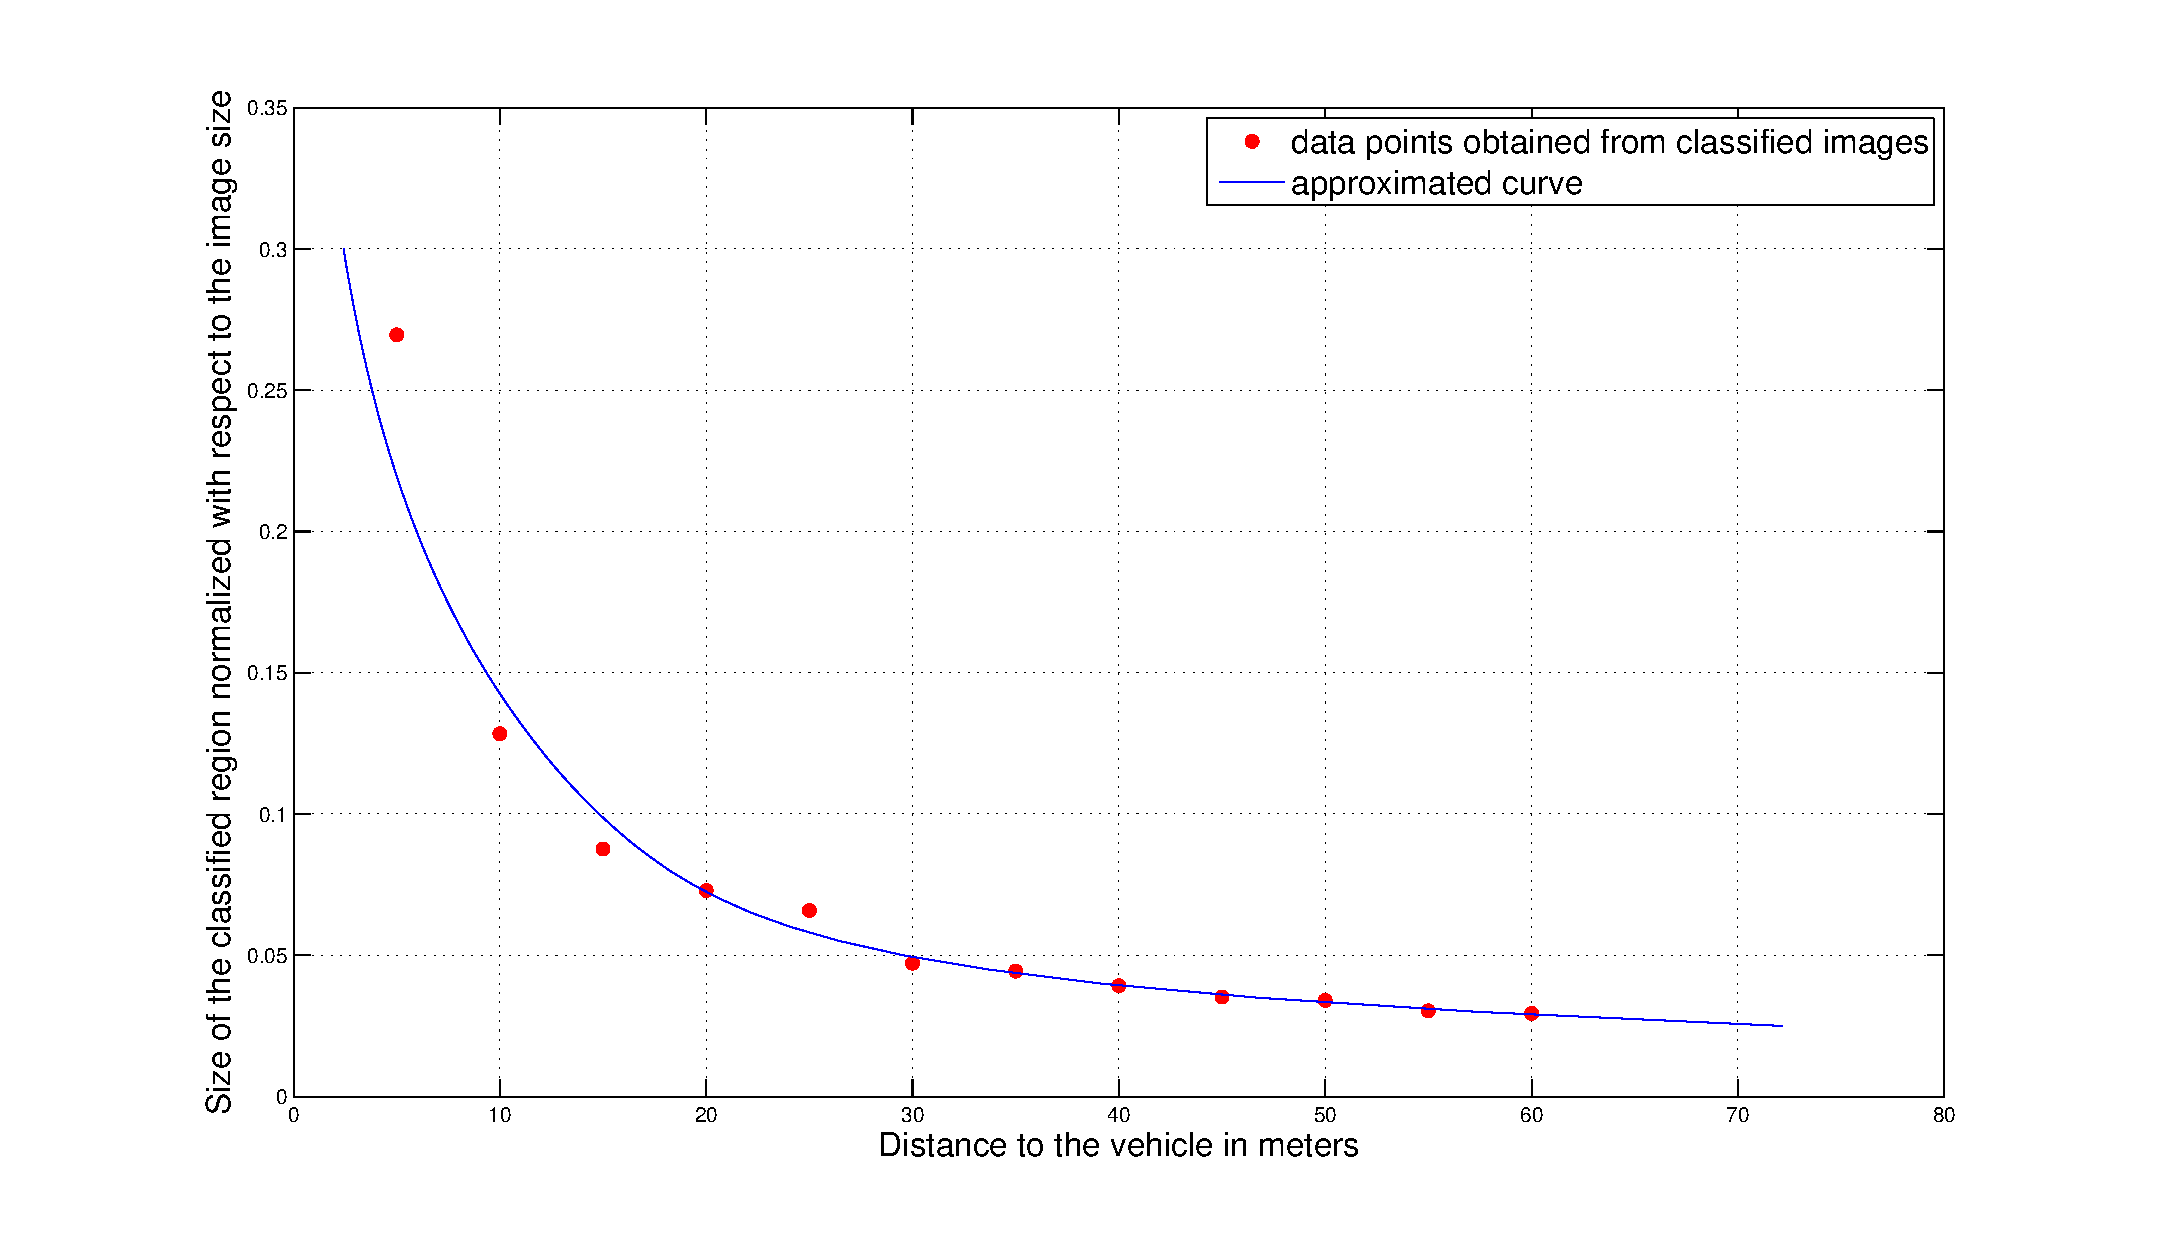
\includegraphics[width=\linewidth]{img/fitted_curve.eps}
\caption{This image shows the curve approximated to the measurements obtained
from the pictures. In the horizontal axis is the width in pixels of
the classification bounding box around the vehicle. In the vertical axis is the
distance in meters to the vehicle. The red points represent the measure obtained
from each image. The blue curve is the predicting model fitted to the data points.}
\label{fig:distance-curve-fitting}
\end{figure} 

It is important to point out that this approximated model is directly related to
the classifier itself. This is because the measurements from the pictures are
obtained through it. This implies that whenever the classifier is changed, a new
coefficients are need to be found.

These coefficients creates a relationship between the width in pixels
of the classified image of the vehicle with the distance in meters to the
vehicle in the real world. Therefore they offer an approximated distance to the
vehicle, giving an initial solution to the problem of distance estimation.

% section Distance estimation (end)


%ERGEBNISSE

\chapter{Bibtex, Citavi und Zitieren} \label{kap:bibtex}
Diese LaTeX-Vorlage verwendet Bibtex zur einfachen Darstellung eines Literaturverzeichnisses.

Es gibt verschiedene Editoren f�r Bibtex Dateien, z.B. JabRef.

Wird mit Citavi gearbeitet, so kann die Literatur automatisch in eine Bibtex-Datei geschrieben werden. \\

Daf�r auf Datei -> Exportieren

\begin{figure}[h]
	\centering
\includegraphics[width=12cm]{img/bib1.png}
\caption{\textit{Exportieren}}
\label{fig:bib1}
\end{figure} 

Im n�chsten Fenster auf "Alle XX Titel in diesem Projekt" und "Weiter".\\

Anschlie�end "BibTeX" anw�hlen und "Weiter".

\begin{figure}[!ht]
	\centering
\includegraphics[width=13cm]{img/bib2.png}
\caption{\textit{Fomart zum Exportieren}}
\label{fig:bib2}
\end{figure} 

Jetzt die entsprechende *.bib Datei ausw�hlen. Diese sollte in dem Projektordner liegen und Bibtex.bib hei�en. F�r einen anderen Ort oder Dateinamen muss "$\backslash$bibliography\{Bibtex\}" im "Studienarbeit.tex" entsprechend angepasst werden.
Au�erdem einen Haken bei "Bibtex-Datei aktualisieren".

\begin{figure}[!ht]
	\centering
\includegraphics[width=13cm]{img/bib3.png}
\caption{\textit{Datei ausw�hlen}}
\label{fig:bib3}
\end{figure} 

Im n�chsten Fenster der Exportvorlage einen Namen geben und einen Haken bei "Automatisch exportieren beim Speichern" setzen. 

\begin{figure}[ht]
	\centering
\includegraphics[width=13cm]{img/bib4.png}
\caption{\textit{Automatisch aktualisieren}}
\label{fig:bib4}
\end{figure} 

Bei jeder �nderung in Citavi aktualisiert sich die Bibtex-Datei automatisch mit und ist somit immer auf dem aktuellstem Stand. 

Die gesamte in Citavi gespeicherte Literatur steht nun zum zitieren bereit und es kann mit "$\backslash$cite\{Name.Jahr\}" eine Literaturangabe gesetzt werden. Damit alle Zitate und Seitenzahlen stimmen, muss das Projekt am Ende mehrfach kompiliert werden.\\

Beispiel:

So sagte \cite{Mustermann.2012}, dass... bzw. "Ich bin klug" \citep{Mustermann.2012}.





% --------------------------------------------------
% -------------- LITERATURVERZEICHNIS --------------
% --------------------------------------------------
	
	
\bibliographystyle{apalike} %Zitierstil wie APA6
\bibliography{Bibtex} %Bibliotheksdatei, hier Bibtex.bib



% --------------------------------------------------
% ------------------ VERZEICHNISSE -----------------
% --------------------------------------------------


\listoffigures %Abbildungsverteichnis
\listoftables %Tabellenverzeichnis



% --------------------------------------------------
% --------------------- GOSSAR ---------------------
% --------------------------------------------------


%Sollte ein Glossar erw�nscht sein:
\addcontentsline{toc}{chapter}{Glossar}
\chapter*{Glossar}
\begin{tabbing}
\hspace{3cm} \= \hspace{10cm} \kill \\
MfG \> Mit freundlichen Gr��en\\
\end{tabbing}
 %Bitte bearbeiten




% --------------------------------------------------
% -------------------- ANHANG ----------------------
% --------------------------------------------------


\begin{appendix} %Anhang
\refstepcounter{chapter}
\addchap{Anhang}
Anhang A 

\end{appendix}

\end{document}

% --------------------------------------------------
% --------------------------------------------------
% --------------------------------------------------
